%  Copyright (C) 2003 David Roundy
%
%  This program is free software; you can redistribute it and/or modify
%  it under the terms of the GNU General Public License as published by
%  the Free Software Foundation; either version 2, or (at your option)
%  any later version.
%
%  This program is distributed in the hope that it will be useful,
%  but WITHOUT ANY WARRANTY; without even the implied warranty of
%  MERCHANTABILITY or FITNESS FOR A PARTICULAR PURPOSE.  See the
%  GNU General Public License for more details.
%
%  You should have received a copy of the GNU General Public License
%  along with this program; if not, write to the Free Software Foundation,
%  Inc., 59 Temple Place - Suite 330, Boston, MA 02111-1307, USA.  
\documentclass[floats]{report}
\usepackage{color}
\usepackage{epsfig}
\usepackage{amsmath, amsthm, amssymb}

\usepackage{verbatim}
\usepackage{html}

\begin{document}

% Definition of title page:
\title{
    Dactyl\\
{\Large \it CYLindrical Time DomAin}
}
\author{
    David Roundy, Mihai Ibanescu, Peter Bermel
}

\maketitle 

\tableofcontents

\chapter{The Yee lattice}

\begin{figure}
\caption{Yee lattice in cylindrical coordinates.
\label{yee_fig}}
\centering
\mbox{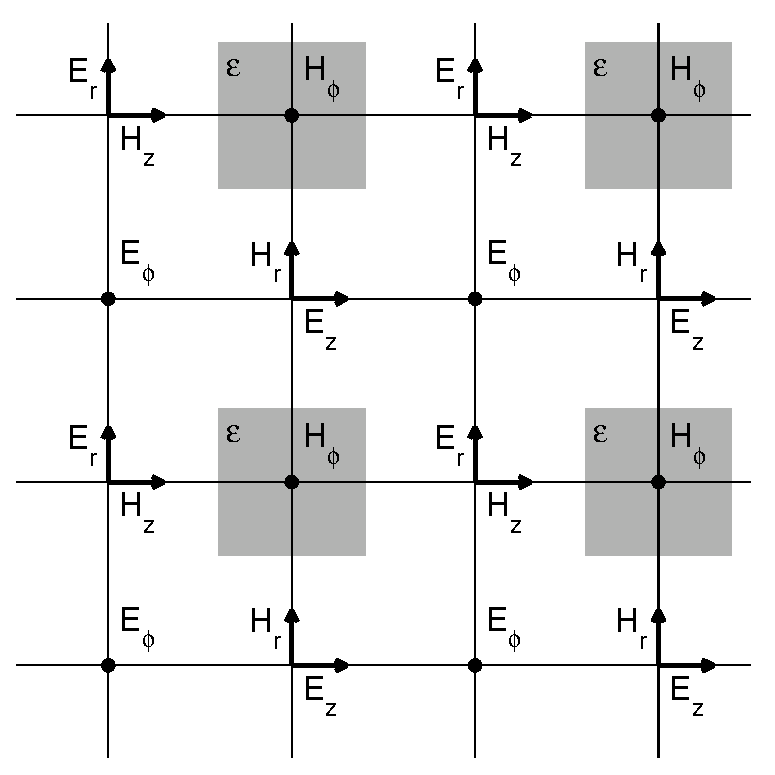
\epsfig{file=Yee_bulk.eps,width=7.8cm}}
\vspace{13cm}
\end{figure}

\chapter{Maxwell's equations in cylindrical coordinates}

Here are Maxwell's equations in cylindrical coordinates.  We take the
fields to be of the form:
\begin{equation*}
\mathbf{E}(r,\phi,z) = \mathbf{E}_m(r,z)e^{i m \phi} 
\end{equation*}

Without further ado:
\begin{align}
\frac1c\frac{dH_r}{dt} &= \frac{dE_\phi}{dz} - \frac{im}r E_z\\
\frac1c\frac{dH_\phi}{dt} &= \frac{dE_z}{dr} - \frac{dE_r}{dz}\\
\frac1c\frac{dH_z}{dt} &= \frac{im}r E_r - \frac1r\frac{d(rE_\phi)}{dr}
\end{align}
\begin{align}
\frac\epsilon c\frac{dE_r}{dt} &= \frac{im}r H_z - \frac{dH_\phi}{dz} \\
\frac\epsilon c\frac{dE_\phi}{dt} &= \frac{dH_r}{dz} - \frac{dH_z}{dr} \\
\frac\epsilon c\frac{dE_z}{dt} &= \frac1r\frac{d(rH_\phi)}{dr} - \frac{im}r H_r
\end{align}


\chapter{PML}

PML (Perfectly Matched Layers) is used to provide absorbing boundary
conditions in either the $z$ or $r$ direction.  PML consists of a material
in which some of the field components are split into two fields, each of
which has a conductivity associated with it, which is responsible for the
absorption of the PML.

PML is a sort of material that contains a set of conductivities $\sigma_r$,
$\sigma_\phi$ and $\sigma_z$.  These conductivities are both $\mathbf{E}$
and $\mathbf{H}$ conductivities---yes, we have magnetic monopoles moving
around in our PML.  $\ddot\smile$ Each $\sigma$ causes absorption of
radiation in the direction it is named after.  Thus $\sigma_\phi$ is small,
and almost unnecesary, and is only needed because of the curvature of the
radial surface.  The value of $\sigma_\phi$ at a given radius is equal to
\begin{equation}
\sigma_\phi(r) = \frac1r \int_0^r \sigma_r(r)dr
\end{equation}

If we had a IDTD (Infinitesimal Difference Time Domain) code, PML would be
perfectly absorbing, regardless of the variation of $\sigma$ with position.
However, since dactyl is a lowly FDTD code, we have to make sure that
$\sigma$ varies only slowly from one grid point to the next.  We do this by
making $\sigma_z$ (for example) vary as $z^2$, with a maximum value of
$\sigma_{max}$ right in front of the boundary.  At the edge of the PML
region is a metalic boundary condition.  The optimal value of
$\sigma_{max}$ is determined by a tradeoff between reflection off the
metallic boundary, caused by too little a $\sigma_{max}$, and reflection
off the sigma itself, caused by too large a $\sigma_{max}$, which makes for
a large variation of $\sigma$ from one grid point to the next.

Here are the field equations for a PML material:
\begin{align}
\frac{dH_{r\phi}}{dt} &= - c \frac{im}r E_z             - \sigma_\phi H_{r\phi} &
\frac{dH_{rz}}{dt} &= c \frac{dE_\phi}{dz}              - \sigma_z H_{rz}\\
\frac{dH_{\phi z}}{dt} &= - c \frac{dE_r}{dz}           - \sigma_z H_{\phi z} &
\frac{dH_{\phi r}}{dt} &= c \frac{dE_z}{dr}             - \sigma_r H_{\phi r} \\
\frac{dH_{zr}}{dt} &= - c \frac1r\frac{d(rE_\phi)}{dr}  - \sigma_r H_{zr}  &
\frac{dH_{z\phi}}{dt} &= c \frac{im}r E_r               - \sigma_\phi H_{z\phi} \\
\epsilon\frac{dE_{r\phi}}{dt} &=   c \frac{im}r H_z             - \sigma_\phi E_{r\phi} &
\epsilon\frac{dE_{rz}}{dt} &= -c\frac{dH_\phi}{dz}              - \sigma_z E_{rz}\\
\epsilon\frac{dE_{\phi z}}{dt} &=   c \frac{dH_r}{dz}           - \sigma_z E_{\phi z} &
\epsilon\frac{dE_{\phi r}}{dt} &=-c \frac{dH_z}{dr}             - \sigma_r E_{\phi r} \\
\epsilon\frac{dE_{zr}}{dt} &=   c \frac1r\frac{d(rH_\phi)}{dr}  - \sigma_r E_{zr}  &
\epsilon\frac{dE_{z\phi}}{dt} &=-c \frac{im}r H_r               - \sigma_\phi E_{z\phi} 
\end{align}

\chapter{Of polaritons and plasmons}\label{polaritons}

Most real materials, at least in some frequency range, have polarizations
that are not actually instantaneously proportional to the local electric
field.  We model these polaritonic and plasmonic effects by introducing one
or more additional polarization fields, to be propogated along with the
electric and magnetic field.  The polarization field, $\mathbf{P}$, is a
vector field which exists on the electric field Yee lattice points.

The polarization field obeys a second order differential equation, which
means that we need to keep track of the polarization at two time steps, in
order to integrate it.

\begin{equation}
\frac{d^2\mathbf{P}}{dt^2} + \gamma \frac{d\mathbf{P}}{dt}
+ \omega^2 \mathbf{P} = \Delta\epsilon\ \omega^2 \mathbf{E}
\end{equation}

To this, we need add one more term to maxwell's equation for $\mathbf E$:

\begin{equation}
c \nabla \times \mathbf{H} = \epsilon_\infty \frac{d\mathbf{E}}{dt}
 + \frac{d\mathbf{P}}{dt}
\end{equation}

So far, the polarization is beautifully simple.  However, we would love to
be able to put polaritonic materials into our PML regions, and
unfortunately in the PML region the electric field has been split into two
components, so we need to figure out which of the two components gets the
contribution from $\frac{d\mathbf{P}}{dt}$.  The obvious solution to this
(well, maybe not exactly obvious, but it is the solution) is to split the
polarization field also into two components in the PML region, just as we
split the electric and magnetic fields.

The electric field propogation equations in PML then become:
\begin{align}
\epsilon\frac{dE_{r\phi}}{dt} &=   c \frac{im}r H_z
             - \sigma_\phi E_{r\phi} - \frac{dP_{r\phi}}{dt} \\
\epsilon\frac{dE_{\phi z}}{dt} &=   c \frac{dH_r}{dz}
             - \sigma_z E_{\phi z} - \frac{dP_{\phi z}}{dt} \\
\epsilon\frac{dE_{zr}}{dt} &=   c \frac1r\frac{d(rH_\phi)}{dr}
             - \sigma_r E_{zr} - \frac{dP_{zr}}{dt}
\end{align}
\begin{align}
\epsilon\frac{dE_{rz}}{dt} &= -c\frac{dH_\phi}{dz}
             - \sigma_z E_{rz} - \frac{dP_{rz}}{dt}\\
\epsilon\frac{dE_{\phi r}}{dt} &=-c \frac{dH_z}{dr}
             - \sigma_r E_{\phi r} - \frac{dP_{\phi r}}{dt} \\
\epsilon\frac{dE_{z\phi}}{dt} &=-c \frac{im}r H_r \label{polariton_pml}
             - \sigma_\phi E_{z\phi} - \frac{dP_{z\phi}}{dt}
\end{align}

\chapter{Hints for writing finite difference time domain code}

(Or \emph{Things I forgot many times, so I wrote down so maybe I won't make
  the same mistake again.})

There is just one rule to remember when writing time domain code, and that
is (as Lefteris has repeatedly told me) ``Always know \emph{when} each
equation is evaluated.''  The trick, of course, lies in knowing how to
apply this rule, and remembering to actually apply it (and I think the
latter is perhaps harder than the former).

As an example, I'll convert a PML polariton equation into a finite
difference equation taken from equation~\ref{polariton_pml} of
chapter~\ref{polaritons}.
\begin{equation*}
\epsilon\frac{dE_{z\phi}}{dt} = -c \frac{im}r H_r
             - \sigma_\phi E_{z\phi} - \frac{dP_{z\phi}}{dt}
\end{equation*}
If we consider the $\mathbf{E}$ timesteps to be at times $n$, $n+1$ etc.,
then this equation needs to be evaluated at time $n+\frac12$.  This is no
problem for most of the terms, but it means that the $\sigma_\phi
E_{z\phi}$ term needs to be an average of its values at time $n$ and
$n+1$.  In short (taking $\Delta t$ to be unity)...
\begin{equation*}
\epsilon (E_{z\phi}^{n+1} - E_{z\phi}^n) = -c \frac{im}r H_r^{n+\frac12}
  - \sigma_\phi ( E_{z\phi}^{n+1} + E_{z\phi}^n) - (dP_{z\phi}^{n+1} - dP_{z\phi}^n)
\end{equation*}
Simplifying a tad gives
\begin{equation*}
E_{z\phi}^{n+1} - E_{z\phi}^n = \frac1{\epsilon + \frac12\sigma_\phi}
    \left(-c \frac{im}r H_r^{n+\frac12}
  - \sigma_\phi E_{z\phi}^n - (dP_{z\phi}^{n+1} - dP_{z\phi}^n)\right)
\end{equation*}
Basically, that is all there is to it.  You now have the equation to
determine $E_{z\phi}^{n+1}$ from $E_{z\phi}^n$, $\frac{im}r
H_r^{n+\frac12}$, $dP_{z\phi}^{n+1}$ and $dP_{z\phi}^n$.

\chapter{Tutorial}

\begin{comment}
/*
\end{comment}
\section{Baby's First Bandstructure}
\begin{comment}
*/
\end{comment}

\begin{comment}
#include <stdio.h>
#include <stdlib.h>
#include "dactyl.h"

double eps(const vec &) {
  return 1.0;
}
const int rad = 10;
const int ttot = 1500*rad;
\end{comment}

In this example we calculate the lowest four TE modes of a simple hollow
metallic waveguide of radius one.

\begin{verbatim}
int main(int argc, char *argv[]) {
  initialize(argc, argv);
  FILE *ban = fopen("bands", "w");
  mat ma(volcyl(1.0, 0.0, rad), eps);
  for (int m=0;m<3;m++) {
    for (double k=0.0; k<= 1.01; k += 0.25) {
      master_printf("Working on k of %g and m = %d with a=%d...\n",
                    k, m, rad);
      fields f(&ma, m);
      f.use_bloch(k);
\end{verbatim}

There are a few tricks you should know before you decide to go about
calculating a band structure.  One of the biggest problems in calculating a
band structure in a time domain code is that of exciting all the modes you
are interested in.  dactyl makes this easy with a couple of ``fields''
methods, \verb-initialize_with_n_te-, and \verb-initialize_with_n_tm-.
These initialize the field with the n lowest TE and TM modes respectively.

\begin{verbatim}
      f.initialize_with_n_te(4);
\end{verbatim}

The band structure code itself begins with a call to
\verb-prepare_for_bands-, which allocates space to store the field
data, which is later used for the band structure calculation.  Its third
argument is the maximum frequency you are interested in.

\begin{verbatim}
      double fmax = 1.0, qmin = 200;
      f.prepare_for_bands(0, ttot, fmax, qmin);
      for (int t=0;t<ttot;t++) {
\end{verbatim}

The second band structure function is \verb-record_bands-, which just
copies the fields into the already allocated arrays for future use.

\begin{verbatim}
        f.record_bands();
        f.step();
      }
\end{verbatim}

Finally, the band structure is actually computed and output by the method
\verb-output_bands-.  The key thing to know about
\verb-output_bands- is that its last argument should be something like
twice the number of modes which have a frequency below your maximum.
Rounding this number up slows the code down considerably, but can sometimes
fix problems where harminv (which is used internally) doesn't find the
modes correctly.  Usually, however, when harminv fails it means you are
misunderstanding something (for example, fmax may be less than the lowest
frequency mode).

\begin{verbatim}
      f.output_bands(ban, "band", 35);
    }
  }
  fclose(ban);
  finished();
}
\end{verbatim}


\begin{comment}
#include <stdio.h>
#include <stdlib.h>

#include <meep.h>
using namespace meep;

const int a = 10;
\end{comment}

\section{Computing the band structure of an omniguide}

In this section we give as an example of a more complicated band structure,
a computation of the band structure of an omniguide.  The output of this
program is shown in Figure~\ref{omniguidebands}.

\begin{verbatim}
const int num_layers = 3;
const double rcore = 3.0;

double guided_eps(const vec &v) {
  double rr = v.r() - rcore;
  if (rr > num_layers + 0.3) return 1.0; // outside the entire waveguide
  if (rr < 0.0) return 1.0;   // vacuum in the core
  while (rr > 1.0) rr -= 1.0; // calculate (r - rcore) % 1
  if (rr < 0.3) return 21.16; // in the high dielectric
  return 1.6*1.6;             // in the low dielectric
}
double vacuum_eps(const vec &v) { return 1.0; }
\end{verbatim}

\begin{comment}
int main(int argc, char **argv) {
  initialize mpi(argc, argv);
  deal_with_ctrl_c();
  printf("Running omniguide!\n");

  const double ttot = 1000.0;
  structure s(volcyl(rcore + num_layers + 0.3, 0.0, a), guided_eps);
  const char *dirname = make_output_directory(__FILE__);
\end{comment}

For this band structure example, we use the grace object to create our
plot.
\begin{verbatim}
  grace g("bands", dirname);
  g.set_range(0.0, 0.35, 0.0, 0.35);
\end{verbatim}
\begin{comment}
  s.set_output_directory(dirname);
  structure vac(&s);
  vac.set_epsilon(vacuum_eps);
\end{comment}

Since the m = 0 modes are pure TE or TM, it makes sense to calculate the
two polarizations separately.  Not only does this give us more interesting
output, but it doesn't cost us any time, to speak of, and actually makes
the band structure much easier to converge.  However, for brevity, I won't
include here in the manual computation of the TM modes, but will skip
straight to the TE modes.

\begin{comment}
  {
    const int m=0;
    g.new_set();
    g.set_legend("m = 0, TM");
    for (double k=0.0;k<0.356 && !interrupt;k+=0.05) {
      char k_and_m[10];
      snprintf(k_and_m, 10, "%g-%d", k, m);
      printf("Working on k of %g and m=0 TM with a=%d...\n", k, a);
      fields f(&vac, m);
      f.use_bloch(k);
      f.verbose(1);
      f.phase_in_material(&s, 1000);
      f.initialize_with_n_tm(9);
      double next_slice_time = 0.0;
      while (f.is_phasing() && !interrupt) f.step();
      f.prepare_for_bands(veccyl(4.801,0.0), ttot, .40, 300, 0.0);
      f.prepare_for_bands(veccyl(3.801,0.0), ttot, .40, 300, 0.0);
      f.prepare_for_bands(veccyl(3.301,0.0), ttot, .40, 300, 0.0);
      const double stoptime = f.time() + ttot;
      while (f.time() < stoptime && !interrupt) {
        f.record_bands();
        f.step();
      }
      f.grace_bands(&g, 40);
    }
  }
\end{comment}

\begin{figure}
\label{omniguidebands}
\caption{Omniguide band structure.}
\includegraphics[width=8.8cm,clip=true]{omniguide-out/bands}
\end{figure}

\begin{verbatim}
  for (int m=0;m<2 && !interrupt;m++) {
    g.new_set();
    char m_string[30];
    if (m) snprintf(m_string, 30, "m = %d", m);
    else snprintf(m_string, 30, "m = 0, TE");
    g.set_legend(m_string);
    for (double k=0.0;k<0.351 && !interrupt;k+=0.05) {
\end{verbatim}
In order to populate the modes that we are interested in, we first populate
the modes of an empty waveguide (whose modes are known), and then
adiabatically transform from that waveguide into our omniguide structure.
\begin{verbatim}
      printf("Working on k of %g and %s with a=%d...\n", k, m_string, a);
      fields f(&vac, m);
      f.use_bloch(k);
      f.verbose(1);
      f.phase_in_material(&s, 1000);
\end{verbatim}
We initialize the fields with both TE and TM modes, and then phase in the
epsilon as usual, and then do the actual phasing in of the structure.
\begin{verbatim}
      f.initialize_with_n_te(9);
      if (m) f.initialize_with_n_tm(9);
      while (f.is_phasing() && !interrupt) f.step();
\end{verbatim}
Again, the band structure code is pretty normal, with the only real
difference being that in this case we \emph{really} want to have specify a
large $Q_{min}$, to help meep to distinguish between real modes and
spurious noise.  Note that we are using metallic boundary conditions, so
all physical modes should have infinite lifetime.
\begin{verbatim}
      f.prepare_for_bands(veccyl(4.801,0.0), ttot, .35, 300, 0.0);
      f.prepare_for_bands(veccyl(1.801,0.0), ttot, .35, 300, 0.0);
      f.prepare_for_bands(veccyl(2.801,0.0), ttot, .35, 300, 0.0);
      const double stoptime = f.time() + ttot;
      while (f.time() < stoptime && !interrupt) {
        f.record_bands();
        f.step();
      }
\end{verbatim}
Finally, we just need to compute and output the bands.  We are careful here
to keep in mind that when $m > 0$, there are twice as many bands, since
there are both TM and TE modes.
\begin{verbatim}
      f.grace_bands(&g, m?80:40);
    }
\end{verbatim}
The band is actually printed to disk only when the grace object is
destroyed, which in this case happens just before the program exits.
\begin{comment}
  }
}
\end{comment}

\section{Band structure of a polariton}

\begin{comment}
#include <stdio.h>
#include <stdlib.h>
#include <signal.h>

#include "dactyl.h"

static int stopnow = 0;
void handle_control_c(int i) {
  printf("Be patient, I'll stop as soon as it's convenient...\n");
  stopnow = 1;
}

const double rmax = 1.0;
\end{comment}

Here we compute and plot the band structure of a polariton material.  We
look at a simple metallic waveguide filled with a polaritonic material.
The material we look at has an epsilon of 13.4 and a longitudinal phonon
frequency of 0.7 and a transverse phonon frequency of 0.4.

\begin{figure}
\label{polaritonbands}
\caption{Polariton band structure.}
\epsfig{file=polaritonbands.eps,width=7.8cm,angle=270}
\end{figure}

\begin{verbatim}
double eps(double r, double z) { return 13.4; }
double one(double r, double z) { return 1; }
\end{verbatim}

\begin{comment}
int main(int argc, char **argv) {
  signal(SIGINT, handle_control_c);
  const int rad = 10;
  const int m = 0;
  double k;
  const int ttot = 1000*rad;  
\end{comment}

\begin{comment}
  mat ma(eps, rmax, 0.0, rad);
  const char *dirname = make_output_directory(argv[0]);
  printf("Storing output in directory %s/\n", dirname);
  FILE *ban = create_output_file(dirname, "bands");
  ma.set_output_directory(dirname);
\end{comment}

To create the polaritonic material, we add the polarizability to the
material after we have created it.

\begin{verbatim}
  ma.add_polarizability(one, 0.4, 0.01, 27.63);//0.1);//
\end{verbatim}

In order to easily calculate the bandstructure, we start out with a simple
material with a material with the same epsilon and polarization
frequencies, but with no coupling between the phonons and the
electromagnetic fields.

\begin{verbatim}
  mat vac(&ma);
  vac.make_average_eps();
  vac.add_polarizability(one, 0.4, 0.01, 0.0);
  for (k=0.0;k<30.01 && !stopnow;k+=2.5) {
    printf("Working on k of %g and m = %d...\n", k, m);
    fields f(&vac, m);
    f.use_bloch(k);
\end{verbatim}

We will rather quickly move from this fake material to the actual
polaritonic material.

\begin{verbatim}
    f.phase_in_material(&ma, 10);
\end{verbatim}

Now we excite the first TE mode (we're only looking at m = 0 here), and
remember to excite along with it the phonon with which it couples.

\begin{verbatim}
    f.initialize_with_nth_te(1);
    f.initialize_polarizations();
\end{verbatim}

Finally, we compute the band structure as usual.

\begin{verbatim}
    while (f.is_phasing()) f.step();
    f.prepare_for_bands(0, ttot, .7+0.5*k/30.0, 30);
    
    for (int t=0; t < ttot+1 && !stopnow; t++) {
      f.record_bands();
      f.step();
    }
    f.output_bands(ban, "band", 16);
\end{verbatim}
\begin{comment}
    fflush(ban);
  }
  fclose(ban);
}
\end{comment}

The final output of this routine (as calculated using the ``plot'' program)
is shown in Figure~\ref{polaritonbands}.


\begin{comment}
#include <stdio.h>
#include <stdlib.h>
#include <signal.h>

#include "dactyl.h"
\end{comment}

\section{Computing epsilon of a polaritonic material}

In this example, we compute epsilon as a function of frequency for a simple
polaritonic material.

\begin{figure}
\label{epsilon_polariton}
\caption{Epsilon of a polaritonic material.}
\epsfig{file=epsilon_polariton.eps,width=8.8cm}
\end{figure}

In order to calculate epsilon, we want to generate a simple plane wave.
Unfortunately, a simple plane wave is anything but simple in cylindrical
coordinates.  We approximate one by using a cell with a large radius but
which is small in the z direction.  We then use a plane wave source (one of
the source options in dactyl) with a gaussian profile.  In order to use a
plane wave source, $m$ obviously has to be 1.  If this isn't obvious to
you, think about it for a moment.

One thing to be aware of when using polaritonic materials, is that
generally you will be needing a rather higher grid resolution than you may
be used to in order to properly model the material.  Here I am using an $a$
of just 20, and if you look at figure~\ref{epsilon_polariton}, you can see
that the curve deviates significantly from the predicted result, which
would be essentially symmetric around the resonant frequency of $0.4$.

\begin{verbatim}
const double rmax  = 2.0;
const int rad = 20;
const int npml = 16;
const double pml_thickness = npml/(double)rad;
const double zsize = (4+2*npml)/(double)rad;
const int m = 1;

complex<double> source_broad(double r) {
  double sig = rmax*0.3;
  return exp(-r*r/(2*sig*sig));
}
\end{verbatim}

For our example polaritonic material, we'll use an $\epsilon(0)$ of 13.4.

\begin{verbatim}
double eps(double r, double z) { return 13.4; }
\end{verbatim}
\begin{comment}
double one(double r, double z) { return 1; }

int main(int argc, char **argv) {
  deal_with_ctrl_c();
  const double ttot = 600.0;
  mat ma(eps, rmax + npml/(double)rad, zsize, rad);
  const char *dirname = make_output_directory(argv[0]);
  printf("Storing output in directory %s/\n", dirname);
  ma.set_output_directory(dirname);
\end{comment}
We use PML in both directions.  Note that the polaritonic material will be
within the PML.  This is fine.
\begin{verbatim}
  ma.use_pml(pml_thickness, pml_thickness);
  ma.add_polarizability(one, 0.4, 0.01, 27.63);
\end{verbatim}
\begin{comment}
  fields f(&ma, m);
\end{comment}
We use several plane wave sources, to cover a broad frequency range
(probably we really only need one).
\begin{verbatim}
  double sourceloc = (npml+1.0)/(double)rad;
  f.add_plane_source(0.6 , 0.8, 0.0, 8.0, sourceloc+0.0, source_broad);
  f.add_plane_source(0.4 , 0.8, 0.0, 8.0, sourceloc+0.0, source_broad);
  f.add_plane_source(0.33, 0.8, 0.0, 8.0, sourceloc+0.0, source_broad);
\end{verbatim}
\begin{comment}
  printf("Working on m = %d with a=%d...\n", m, rad);
\end{comment}
We use a couple of monitor points to determine epsilon.
\begin{verbatim}
  monitor_point *left = NULL, *right = NULL;
\end{verbatim}
\begin{comment}
  double next_printtime = 50;
  while (f.time() < ttot && !interrupt) {
    if (f.time() >= next_printtime) {
      next_printtime += 50;
      printf("Working on time %lg...  ", f.time());
      printf("energy is %lg\n", f.total_energy());
    }
\end{comment}
The monitor points are located one grid spacing from one another.  The
\verb*|get_new_point| method appends the fields at a given time to a
monitor point linked list.
\begin{verbatim}
    left  = f.get_new_point(0.2, sourceloc+1.0/rad, left );
    right = f.get_new_point(0.2, sourceloc+2.0/rad, right);
\end{verbatim}
\begin{comment}
    f.step();
  }
  grace g("eps", dirname);
  complex<double> *al, *ar, *freqs;
  int numl, numr;
  printf("Working on left fourier transform...\n");
\end{comment}
When the time stepping is over, we take a fourier transform of the fields
at the two monitor points.
\begin{verbatim}
  left->fourier_transform(Ep, &al, &freqs, &numl, 0.301, 0.5, 1000);
\end{verbatim}
\begin{comment}
  delete[] freqs;
  printf("Working on right fourier transform...\n");
\end{comment}
\begin{verbatim}
  right->fourier_transform(Ep, &ar, &freqs, &numr, 0.301, 0.5, 1000);
\end{verbatim}
\begin{comment}
  if (numl != numr) printf("Aaack you need both nums to be the same!\n");
  g.new_set();
  g.set_legend("\\x\\e\\s2\\N");
\end{comment}
Finally we calculate the complex index of refraction using the equation
\begin{equation*}
i \omega \Delta x n(\omega) = \log \left(\frac{E'(\omega)}{E(\omega)}\right)
\end{equation*}
\begin{verbatim}
  for (int i=0;i<numl;i++) {
    complex<double> I = complex<double>(0,1);
    complex<double> n = (log(ar[i]/al[i]))/(I*(1.0/rad)*2*pi*freqs[i]);
    g.output_point(real(freqs[i]), real(n*n));
  }
\end{verbatim}
\begin{comment}
  g.new_set();
  g.set_legend("\\x\\e\\s2\\N");
  for (int i=0;i<numl;i++) {
    complex<double> I = complex<double>(0,1);
    complex<double> n = (log(ar[i]/al[i]))/(I*(1.0/rad)*2*pi*freqs[i]);
    g.output_point(real(freqs[i]), imag(n*n));
  }
}
\end{comment}



\input{superluminal_epsilon.tex}

\appendix

\input{gpl.tex}

\end{document}

